\chapter{Administrátorské rozhraní}
\label{4-praxe}

\section{Současná správa uživatelských účtů}
\label{cmd-line}
% https://github.com/gislab-npo/gislab/tree/314fe436e1b65783d65e61000ca6d3f8ba873b2f/system/admin

Aktuálně probíhá správa uživatelských účtů spouštěním shellových skriptů. Všechny příkazy je nutné spouštět pod právem \textit{sudo}. Některé z nich umožňují použití parametrů, pro část jsou dokonce povinné.

Seznam názvů dostupných skriptů pro GIS.lab administraci vrací příkaz \textsf{gislab-help}. Každý jednotlivý příkaz z tohoto soupisu pak lze spustit s příznakem \textsf{-h}, který zobrazí podrobnější nápovědu. Uživatel se dozví, co skript vykoná a za jakých podmínek, jakým způsobem příkaz zapsat do konzole a získá přehled parametrů, které může či musí použít.

Níže jsou popsány skripty pro vytváření uživatelů a skupin, jejich mazání a pro výpis existujících entit, protože souvisí s funkčností, kterou nabízí nové webové rozhraní. Vedle toho existují i další, např. pro zálohování dat nebo upgrade GIS.lab systému.

%TK: tady u těch popisů nevím, jestli dávat někam přesnou podobu příkazu (gislab-adduser [OPTIONS] username)
%přímo jako nadpis (\subsubsection{gislab-adduser...}) nebo někam pod něj? nebo to nepsat vůbec?
%nebo mít u každého konkrétní příkaz: $ sudo gislab-adduser -g User -l GIS.lab -m lab1@gis.lab -p lab lab1 ??

\subsubsection{gislab-adduser}
\begin{itemize}
\item [-g] křestní jméno (povinné)
\item [-l] příjmení (povinné)
\item [-m] email (povinné)
\item [-d] popis (nepovinné)
\item [-p] heslo (nepovinné)
\item [-s] přidat uživateli status administrátora (nepovinné)
\item [-a] přidat uživatele do vybraných skupin (nepovinné)
\end{itemize}
Tento příkaz má několik příznaků, z nichž část je povinná, část nepovinná. Parametr \textsf{-p} musí být použit jako poslední, těsně před názvem uživatele (username), může však být aplikován v různých obměnách. První variantou je \textsf{-p PASSWORD}, která nastaví heslo na hodnotu PASSWORD. Pokud je použit parametr bez argumentu (\textsf{-p}), uživatel je následně dotázán na heslo. V třetím případě je parametr z příkazu kompletně vynechán a heslo je automaticky vygenerováno. Tedy i přestože parametr patří mezi nepovinné, heslo je vždy po doběhnutí skriptu vytvořeno.

Uživatele lze přidat do více skupin zároveň použitím parametru \textsf{-a} a seznamu skupin oddělených od sebe čárkami. Pokud je k účtu přiřazen status administrátora (superuser), tak takový uživatel může na klientských počítačích spouštět operace pod právem \textit{sudo}.

\subsubsection{gislab-moduser}
\begin{itemize}
\item [-a] přidat uživatele do vybrané skupiny
\item [-A] odebrat uživatele z vybrané skupiny
\item [-s] přidat uživateli status administrátora
\item [-S] odebrat uživateli status administrátora
\item [-m] změnit email
\item [-p] změnit heslo
\item [-d] změnit popis
\end{itemize}
Upraví jeden či více atributů. Pokud nebyly předtím definovány, tak je vytvoří. Stejně jako při vytváření uživatelského účtu je možné přidávat a odebírat členství ve skupinách hromadně, jsou-li v seznamu a oddělené čárkami. V případě, že je parametr \textsf{-p} uveden bez argumentu, je heslo vygenerováno automaticky.

\subsubsection{gislab-deluser}
\begin{itemize}
\item [-b] zazálohovat uživatelská data (nepovinné)
\item [-f] vynutit proběhnutí tohoto příkazu (nepovinné)
\end{itemize}
Smaže uživatelský účet včetně příslušnosti ke skupinám. Pokud je příkaz spuštěn s parametrem \textsf{-f}, proběhne vše okamžitě, v opačném případě musí uživatel ještě jednou potvrdit, že si skutečně přeje účet odstranit.

\subsubsection{gislab-addgroup}
\begin{itemize}
\item [-d] popis (nepovinné)
\end{itemize}
Vytvoří skupinu.

\subsubsection{gislab-delgroup}
\begin{itemize}
\item [-f] vynutit proběhnutí tohoto příkazu
\end{itemize}
Smaže skupinu, pokud je prázdná. Existují-li uživatelé, kteří patří do mazané skupiny, vypíše se chybová hláška a skupina zůstane v systému. Nejdříve je potřeba skupinu vyčistit přes \textsf{gislab-moduser} a pak příkaz zopakovat.

Obdobně jako při mazání uživatelského účtu je možné vynutit proběhnutí příkazu bez dalších dotazů. Pokud však zůstali nějací uživatelé ve skupině, je vrácena stejná chyba, která byla popsána výše.

\subsubsection{gislab-listusers}
\begin{itemize}
\item [-g] vypsat pouze uživatele zvolené skupiny
\end{itemize}
Bez příznaku vypíše seznam všech uživatelů. U každého uživatele jsou uvedeny všechny jeho atributy. S příznakem \textsf{-g nazev\_skupiny} vypíše list uživatelů příslušících této skupině, včetně jejich atributů. Heslo je zobrazeno v šifrované podobě. 

\subsubsection{gislab-listgroups}
Kromě nápovědy nemá žádné parametry. Vypíše seznam všech skupin a jejich atributů, včetně identifikátorů \textit{uid} uživatelů, kteří do dané skupiny patří. 

Jak \textsf{gislab-listusers}, tak \textsf{gislab-listgroups} vracejí při větším množství záznamů velmi dlouhý seznam, který vypisují do konzole. Zobrazit jen požadovanou část informací umožňuje program grep.

\textsf{\$ sudo gislab-listusers | grep uid:}

\textsf{uid: uid=user01}

\textsf{uid: uid=user02}

%TK: u listusers a listgroups by možná pro lepší orientaci pomohlo přidat obrázky nebo textový výpis, jak vlastně vypadají výsledky, které vrací:
%dn: uid=gislab,ou=People,dc=gis,dc=lab                                                                                  objectClass: inetOrgPerson                                                                                              objectClass: posixAccount                                                                                               objectClass: shadowAccount                                                                                              uid: gislab                                                                                                             uidNumber: 3000                                                                                                         gidNumber: 3001                                                                                                         homeDirectory: /mnt/home/gislab                                                                                         loginShell: /bin/bash                                                                                                   cn: Administrator GIS.lab (gislab_vagrant_bionic)                                                                       sn: GIS.lab (gislab_vagrant_bionic)                                                                                     givenName: Administrator                                                                                                mail: gislab@gis.lab                                                                                                    userPassword:: e1NTSEF9Y0JBWUdMcVgxNTdweVJreXdxZzJRaUlpTE9CaHNaSTU=                                                     description: fjdsklfjdsl 

\section{Webové administrátorské a uživatelské rozhraní}
Technologie použité při vývoji byly zvoleny na základě těch již aplikovaných v rámci platformy GIS.lab, resp. Gisquick. Pro zpracování byl zvolen programovací jazyk Python 3. V první řadě se jedná o budoucnost tohoto jazyka, na rozdíl od Pythonu 2. Také to umožní navázat na nástřel existující knihovny pro správu uživatelů z roku 2015. Navíc je to jazyk, v němž je napsán framework Django, který byl použit také při tvorbě webové aplikace Gisquick. Ta byla původně součástí GIS.labu a tímto způsobem zůstane celá široká základna v jedné technologii.

Pro přístup k \zk{LDAP} serveru bylo třeba vyvíjet konzoli přímo v GIS.labu. Ten běžel ve virtuálním vývojovém prostředí Vagrant, v počátcích na virtuálním serveru Výpočetního a informačního centra ČVUT (\href{gislab-vm.fsv.cvut.cz}{gislab-vm.fsv.cvut.cz}), později na školním počítači (\href{http://b802-01.fsv.cvut.cz}{http://b802-01.fsv.cvut.cz}). 

Django bylo nainstalováno ve virtuálním prostředí, aby nebyl ovlivněn zbytek GIS.labu. Při vývoji webové konzole byl využit odlehčený webový server Djanga (vývojový server) a implicitní databáze SQLite. Pro vytvoření základní struktury projektu a aplikace \textit{users} byly použity vestavěné příkazy Djanga. 

Balíčků pro autentizaci Djanga vůči \zk{LDAP} serveru existuje velké množství. První ze zvažovaných knihoven byla \textit{django-auth-ldap}, která provádí autentizaci uživatelů a při jejich prvním přihlášení vytvoří účet v databázi Djanga. Nakonec byla zvolena knihovna \textit{django\_python3\_ldap}, jež navíc obsahuje možnost vytvořit všechny uživatelské účty zároveň spuštěním příkazu \textsc{manage.py ldap\_sync\_users}. Kromě toho tuto knihovnu využívá i platforma Gisquick\footnote{https://github.com/gislab-npo/gislab/blob/master/system/roles/service-gisquick/files/static/django/settings\_custom.py}, která byla velkou inspirací v počátcích vývoje. \textit{django\_python3\_ldap} navazuje na knihovnu \textit{ldap3}. 

Pro synchronizaci z Djanga do \zk{LDAP} byly provedeny pokusy využít existující knihovny \textit{django-ldapdb} a \textit{django-ldap-user-registration}. Ani jednu se nepodařilo zprovoznit pro potřeby GIS.labu a proto byla vytvořena vlastní třída \textsf{SyncDjangoLDAP}, která také staví na \textit{ldap3}. 

\zk{LDAP} server v původní konfiguraci neumožňuje, aby samotní uživatelé měnili údaje někoho jiného ani své vlastní. Proto byl vytvořen modifikační soubor:

\begin{verbatim}
dn: olcDatabase={1}mdb,cn=config
changetype: modify
add: olcAccess
olcAccess: to * 
  by dn.exact="cn=admin,dc=gis,dc=lab" manage  
  by self write  
  by * read
\end{verbatim}

který do nastavení serveru přidal právo pro správce \textit{cn=admin,dc=gis,dc=lab} upravovat všechny uživatele v databázi, pro všechny uživatele upravovat své vlastní údaje a pro ostatní právo čtení. Stejným způsobem bylo pozměněno již existující nastavení práv k úpravě hesla, kde byly rozšířeny kompetence správce, aby mohl upravovat všechny:

\begin{verbatim}
dn: olcDatabase={1}mdb,cn=config
changetype: modify
delete: olcAccess
olcAccess: {0}
-
add: olcAccess
olcAccess: {0}to attrs=userPassword
  by dn.exact="cn=admin,dc=gis,dc=lab" manage
  by self write
  by anonymous auth
  by * none
\end{verbatim}

Modifikační soubory byly využity při spuštění operace ldapmodify, která slouží k úpravám konfigurace \zk{LDAP} serveru:
\begin{center}
\textsf{sudo ldapmodify -Q -Y EXTERNAL -f /cesta/k/modifikacnimu/souboru}
\end{center}

Změny byly aplikovány restartováním \textit{slapd}:
\begin{center}
\textsf{sudo service slapd restart}
\end{center}

V situaci, kdy jsou upravovány údaje v \zk{LDAP} skrze webovou konzoli, je vytvořeno připojení s přihlašovacími údaji správce \textit{cn=admin,dc=gis,dc=lab}, proto je dostačující nastavit nejvyšší práva pouze pro něj.

Webové rozhraní má dvě hlavní části - uživatelskou a administrátorskou. Administrátorská konzole vychází z vestavěné správcovské konzole Djanga a je upravena potřebám GIS.labu. Uživatelská konzole je vytvořená samostatně. 

%zatim newpage, pak se to pořeší při dolaďování vzhledu
\newpage
\subsection{Struktura projektu}
Adresářová struktura projektu:
% tomuhle budu chtít dát hezčí design
% např. forest: https://tex.stackexchange.com/questions/5073/making-a-simple-directory-tree
% https://tex.stackexchange.com/questions/328886/making-a-directory-tree-of-folders-and-files/328890
\dirtree{%
.1 web\_admin\_console.			
	.2 project.
		.3 \_\_init\_\_.py.
		.3 ldap\_auth.py.
		.3 settings.py.
		.3 settings\_custom.py.
		.3 urls.py.
		.3 wsgi.py.
    .2 static.
    	.3 styles.css.
	.2 templates.
		.3 registration.
			.4 login.html.
		.3 base.html.
		.3 home.html.
		.3 password\_change.html.
		.3 signup.html.
		.3 user\_change.html.
	.2 users.
		.3 templatetags.
			.4 \_\_init\_\_.py.
			.4 auth\_extras.py.
		.3 \_\_init\_\_.py.
		.3 admin.py.
		.3 apps.py.
		.3 forms.py.
		.3 ldap\_sync.py.
		.3 models.py.
		.3 tests.py.
		.3 urls.py.
		.3 views.py.
	.2 db.sqlite3.
	.2 manage.py.
    }

\subsubsection{project}
Základní struktura projektu v Djangu byla vygenerována automaticky po spuštění \textsf{django-admin startproject project} (viz \ref{django-app}).

%settings_custom.py
Doplňující nastavení je definováno v novém souboru \textbf{settings\_custom.py}, který je naimportován na konci původního souboru \textit{settings.py}. V tomto souboru je v první řadě definována \zk{URL} adresa, na které je webová konzole dostupná a zaregistrovány používané aplikace - tedy vlastní aplikace \textit{users} popsaná níže a knihovna \textit{django\_python3\_ldap}, která řídí komunikaci a synchronizaci s \zk{LDAP} serverem. Dále jsou zde určeny cesty k nalezení šablon a statických souborů.

Rovněž je v tomto souboru definován vlastní uživatelský model a autentizační backend využívající \zk{LDAP} server namísto \textit{ModelBackend}, který je pro Django implicitní. Pro správnou funkčnost knihovny \textit{django\_python3\_ldap} jsou nakonfigurovány potřebné proměnné, mezi hlavními \zk{URL} \zk{LDAP} serveru, úroveň, na níž se mají vyhledávat v \zk{LDAP} uživatelé či namapování ekvivalentních atributů mezi \zk{LDAP} a Djangem. Kromě toho je na konci volána vlastní funkce ze souboru \textit{ldap\_auth.py}, jež provádí synchronizaci skupin do Djanga.

%ldap_auth.py
Soubor \textbf{ldap\_auth.py} sestává z jediné funkce \textsf{custom\_sync\_user\_relations()}. Používaná knihovna \textit{django\_python3\_ldap} při synchronizaci předpokládá existenci atributu \textit{MemberOf} u uživatelského záznamu v databázi na \zk{LDAP} serveru. Ten obsahuje informace o skupinách, jichž je uživatel členem. GIS.lab server tento parametr u uživatelů nemá a nastavení nebylo možné změnit, data o příslušnosti jsou ukládána pouze na straně skupin. Proto byla napsána vlastní funkce, která synchronizaci provádí.

Nejdříve je vytvořeno anonymní připojení k \zk{LDAP} serveru a získán seznam existujících skupin. Ty jsou porovnány se skupinami v Djangu a v případě nesrovnalostí je Django aktualizováno podle stavu na \zk{LDAP} serveru. Stejným způsobem je provedena synchronizace členství, kdy jsou postupně procházeny všechny skupiny a je testováno, zda je uživatel jejich členem na \zk{LDAP} serveru. Po doběhnutí této funkce jsou z pohledu skupin Django a \zk{LDAP} konzistentní.

%urls.py
Soubor \textbf{urls.py} v základní podobě obsahuje pouze \zk{URL} adresu k vestavěné administrátorské konzoli Djanga. K ní jsou přidány cesty ke správě uživatelů a k vlastní aplikaci \textit{users} a definována šablona \textit{home.html} jako domovská stránka.

\subsubsection{users}

Tento adresář sestává z souborů tvořících Django aplikaci s názvem \textit{users}, základní struktura byla vytvořena příkazem \textsf{python manage.py startapp users}.

%models
V souboru \textbf{models.py} je definován vlastní uživatelský model \textsf{CustomUser}, který dědí z třídy \textsf{AbstractUser} a rozšiřuje ji o nový textový atribut \textsf{description}.

%forms
\textbf{forms.py} definuje třídy vlastních formulářů, které všechny dědí z vhodných tříd Djanga a přidávají potřebnou funkcionalitu. \textsf{CustomUserCreationForm} slouží k registraci nových uživatelů, \textsf{CustomUserChangeForm} je použit při změně osobních údajů. Oba formuláře mají nastaven model na \textsf{CustomUser} a definován seznam polí, která se zobrazí při registraci, resp. úpravě údajů. V třídě \textsf{FieldsRequiredMixin}, která je předána oběma jako parametr, jsou určeny povinné a nepovinné atributy tak, aby odpovídaly atributům na \zk{LDAP} serveru. Povinné jsou, vedle uživatelského jména a hesla, křestní jméno, příjmení a emailová adresa. Nepovinné pak zůstává pouze pole popisu. U registračního formuláře je navíc přetížena metoda \textit{save()} tak, aby byl při vytváření nový uživatel uložen i na \zk{LDAP} server.

Posledním formulářem je \textsf{CustomAdminPasswordChangeForm}, jenž slouží ke změně hesla. U něj je také přetížená funkce \textit{save()} tak, aby nové heslo bylo upraveno i na serveru.

%admin
V souboru \textbf{admin.py} jsou veškeré změny, které upravují standardní nastavení administrátorské konzole Djanga. Sestává ze dvou tříd, jedné pro správu uživatelů a druhé pro správu skupin (rolí). 

V \textsf{CustomUserAdmin} je připojen vlastní model \textsf{CustomUser} a vlastní formuláře pro vytváření uživatele, změnu údajů a hesla. Implicitní nastavení je upraveno a zobrazují se jen pole a filtry, které jsou pro administrátorskou konzoli potřebné. Při manipulaci s uživatelským účtem přes administrátorskou konzoli se nevolají metody formuláře, ale metody třídy \textsf{UserAdmin}. Proto jsou zde přetíženy metody \textsf{save\_model()}, která vytváří či upravuje uživatele, a \textsf{delete\_model()}, jež uživatele maže. Po úpravě promítají tyto změny také na \zk{LDAP} server.

Podobně upravená je i třída \textsf{CustomGroupAdmin}. Ta sice ponechává původní model \textsf{Group}, ale z atributů je zobrazen jenom název. Metody \textsf{save\_model()} a \textsf{delete\_model()} jsou přetížené stejně jako u administrace uživatelů a změny jsou promítány na \zk{LDAP} server.

Na konci souboru jsou obě vlastní třídy zaregistrovány a popisy v Django administraci jsou upraveny, aby lépe odpovídaly potřebám GIS.lab konzole.

%ldap_sync
%TK:možná by to bylo přehlednější, kdybych tady k tomu připsala nějaký hodně stručný pseudokod? s tím, co se v které metodě synchronizuje?
Soubor \textbf{ldap\_sync.py} je zcela nově vytvořen a obsahuje vlastní třídu \textsf{SyncDjangoLDAP}, jež provádí synchronizaci změn z Djanga do \zk{LDAP}. Při její inicializaci je vytvořeno připojení k \zk{LDAP} serveru s přihlašovacími údaji pro hlavního GIS.lab administrátora se jménem \textit{cn=admin,dc=gis,dc=lab}, heslo je uloženo v textovém souboru. V rámci destruktoru je připojení zrušeno. 

Pro synchronizaci je využita externí knihovna ldap3, konkrétně operace \textsf{ADD}, \textsf{MODIFY} a \textsf{DELETE}. Metoda \textsf{change\_user()} zjistí, která data byla editována, a provede tuto změnu i v \zk{LDAP}. Upravuje nejenom vlastní atributy uživatele, ale i členství ve skupinách. Jen změna hesla má jinou metodu, \textsf{change\_password()}, protože se jedná o atribut, který má vlastní formulář pouze pro heslo. 

Nového uživatele ukládá metoda \textsf{save\_user()}. Některé atributy jsou zvoleny jako konstanty (např. identifikační číslo), protože se jedná o interní hodnoty \zk{LDAP} a v Django neexistuje jejich ekvivalent. Do budoucna by tento problém mělo vyřešit propojení s Python knihovnou pro správu (viz \ref{python-knihovna}). Odstranění účtu řídí \textsf{delete\_user()}, jež nejdřív odstraní všechny vztahy uživatele a pak jej teprve smaže. 

Skupiny lze pouze vytvořit přes \textsf{save\_group()} či odstranit v metodě \textsf{delete\_group()}. Není umožněno provádět žádné úpravy, protože jediným existujícím atributem je název role. Při tvorbě je zvolena konstanta pro identifikační číslo skupiny, propojení s Python knihovnou tuto situaci vyřeší (viz výše). Před odstraněním jsou nejdříve zrušeny veškeré vztahy k uživatelům. 
 
%views
Soubor \textbf{views.py} obsahuje logiku propojující formuláře a modely se zobrazením přes uživatelskou konzoli. Jedná se o tři pohledy (třídy), jeden pro registraci (\textsf{SignUp}), druhý pro úpravu uživatelských údajů (\textsf{ChangeUser}) a třetí pro změnu hesla (\textsf{ChangePassword}). U všech je definováno, který formulář mají použít, ve které šabloně je zobrazen a kam uživatele přesměrovat po správném vyplnění a odeslání. U pohledu editace údajů je přetížená funkce \textsf{form\_valid()} tak, aby navíc volala třídu \textsf{SyncDjangoLDAP} a promítala změny i do \zk{LDAP}.

%urls
Posledním souborem v adresáři \textit{users} je \textbf{urls.py}, jenž definuje \zk{URL} adresy ke třem výše zmiňovaným pohledům - registraci, změně údajů a úpravě hesla.

\subsubsection{templates, templatetags, static}
Složka \textbf{templates} obsahuje šablony (templates), psané v jazyce \zk{HTML}, které umožňují vypisovat vybraná data z modelů do prohlížeče. Cesta k adresáři musí být registrována v souboru \textit{settings.py} v proměnné \textsf{DIRS} u položky \textsf{TEMPLATES}.

Pro přístup k proměnným a některým funkcím Pythonu slouží složené závorky. V případě proměnných se jedná o závorky dvojité: \textsf{\{\{ variable \}\}}. 

%popis sablon
Django funguje na principu dědičnosti. Bázovou šablonou je \textbf{base.html}. Vložením textu \textsf{\{\% extends "base.html" \%\}} na začátek jiné šablony, např. \textit{child.html}, je nejdříve načtena šablona \textit{base.html}, definující základní bloky, a až následně je k nim přidán obsah \textit{child.html}. Tímto způsobem jsou omezeny duplicity v jednotlivých šablonách.

U tohoto projektu jsou například v bázové šabloně definovány navigační prvky společné pro níže uvedené šablony, které z ní všechny dědí. Na každé stránce se v horní části zobrazuje logo GIS.labu, které po kliknutí přesměruje uživatele na hlavní stránku \textit{home.html}. V případě přihlášeného uživatele se navíc zobrazuje tlačítko pro odhlášení.

\textbf{signup.html} obsahuje jednoduchý interaktivní formulář s informacemi, která pole jsou povinná pro platné vyplnění a jaké podmínky musí splňovat. V situaci, kdy je registrace provedena správně, je uživatel přesměrován na přihlašovací stránku, v opačném případě je zobrazena chybová hláška a potřebná data je nutné opravit, resp. doplnit.

Template \textbf{login.html} sestává z jednoduchého formuláře pro vyplnění uživatelského jména a hesla. Při neúspěšném pokusu je vypsána chyba, po zdárném vyplnění je uživatel přesměrován na domovskou stránku \textit{home.html}.

První šablona, s níž se uživatel při zobrazení hlavní stránky setká, je \textbf{home.html}. Ta ukazuje rozdílné výsledky nepřihlášenému uživateli a přihlášenému. V prvním případě je dostupný rozcestník, který jej navede na stránky přihlášení či k registraci. V druhém případě, tedy pokud je již přihlášen, se zobrazí jeho osobní informace a aktivní role. Přímo zde nemůže nic upravovat, ale pomocí tlačítka \textsf{Edit} je přesměrován na stránku s úpravou osobních údajů.

Šablona \textbf{user\_change.html} obsahuje formulář pro editaci osobních údajů, který umožňuje upravit jeden či více záznamů naráz. Heslo se zde nezobrazuje, ale přes odkaz lze pokračovat na stránku \textit{password\_change.html}, kde je možné provést jeho změnu.

%static
Složka \textbf{static} umístěná v hlavním adresáři projektu obsahuje soubor \textit{styles.css}, jenž popisuje způsob zobrazení elementů, které jsou součástí jednotlivých šablon uživatelské konzole. To je umožněno načtením tohoto souboru pomocí \textsf{\{\% load static \%\}} do bázové šablony. K vytvoření designu byly použity kaskádové styly (\zk{CSS}).

%template tags
Django umožňuje vytvořit si vlastní filtry. Ty jsou specifikovány v souboru \textbf{auth\_extras.py} uloženém v adresáři aplikace \textit{users/templatetags} a k šablonám jsou připojeny pomocí \textsf{\{\% load auth\_extras \%\}}. Filtru \textsf{foo} lze předat hodnotu proměnné \textit{var} a argument \textit{arg}. Poté, co je filtr zaregistrován jako \textit{django.template.Library.filter()} a definována žádaná funkce, je možné jej zavolat v šabloně příkazem:

\textsf{\{\{ var|foo:"arg" \}\}}

Pro potřeby zobrazení aktivních rolí uživatele v šabloně \textit{home.html} byly vytvořeny dva filtry. První zjišťuje všechny existující role v databázi Djanga a na něj navazuje druhý, který určuje, zda je uživatel jejich členem. Výsledky jsou pak zobrazeny v \zk{GUI}.

\subsubsection{db.sqlite3}
% https://www.tablesgenerator.com/latex_tables

Pro vývoj byla využita implicitní databáze Djanga SQLite. Z hlediska uživatelů a rolí jsou důležité především tři tabulky \textit{auth\_group}, \textit{users\_customuser} a \textit{users\_customuser\_groups}. 

Tabulka \textbf{auth\_group} obsahuje pouze názvy existujících rolí.

\begin{table}[H]
\centering
\begin{tabular}{@{}|c|c|c|@{}}
\toprule
\multicolumn{3}{|c|}{auth\_group} \\ \midrule
name & id & name \\ \midrule
type & integer & varchar(80) \\ \bottomrule
\end{tabular}
\caption{Atributy tabulky auth\_group}
\label{tab:auth-group}
\end{table}

Tabulka \textbf{users\_customuser} sestává z osobních údajů uživatelů včetně zašifrovaného hesla, data vytvoření, posledního přihlášení a interních statusů Djanga. 

\begin{table}[H]
\centering
\resizebox{\textwidth}{!}{%
\begin{tabular}{@{}|c|c|c|c|c|c|c|@{}}
\toprule
\multicolumn{7}{|c|}{users\_customuser} \\ \midrule
name & id & password & last\_login & is\_superuser & username & first\_name \\ \midrule
type & integer & varchar(128) & datetime & bool & varchar(150) & varchar(30) \\ \bottomrule
\end{tabular}%
}
\caption{Atributy tabulky users\_customuser 1/2}
\label{tab:users-customuser-1}
\end{table}

\begin{table}[H]
\centering
\resizebox{\textwidth}{!}{%
\begin{tabular}{@{}|c|c|c|c|c|c|c|@{}}
\toprule
\multicolumn{7}{|c|}{users\_customuser} \\ \midrule
name & last\_name & email & is\_staff & is\_active & date\_joined & description \\ \midrule
type & varchar(150) & varchar(254) & bool & bool & datetime & text \\ \bottomrule
\end{tabular}%
}
\caption{Atributy tabulky users\_customuser 2/2}
\label{tab:users-customuser-2}
\end{table}

Tabulka \textbf{users\_customuser\_groups} propojuje obě výše zmíněné tabulky, tj. příslušnost uživatelů k jednotlivým skupinám.

\begin{table}[H]
\centering
\begin{tabular}{@{}|c|c|c|c|@{}}
\toprule
\multicolumn{4}{|c|}{users\_customuser\_groups} \\ \midrule
name & id & customuser\_id & group\_id \\ \midrule
type & integer & integer & integer \\ \bottomrule
\end{tabular}
\caption{Atributy tabulky users\_customuser\_groups}
\label{tab:users-customuser-groups}
\end{table}

\subsection{Spuštění projektu}
Ve finální verzi bude webová konzole zaintegrována do GIS.labu pomocí Docker kontejneru jako samostatná služba. Při odevzdání je projekt ještě ve vývojové fázi. Pro jeho spuštění je třeba mít nainstalovanou platformu GIS.lab alespoň ve virtuální režimu. Projekt si uživatel může sestavit sám či může využít připravený skript, který je dostupný v repozitáři. \footnote{https://github.com/ctu-geoforall-lab-projects/dp-kulovana-2019}

Shellový skript \textbf{setup\_script.sh} připraví projekt ke spuštění, jediné co musí uživatel udělat, je upravit proměnnou \textsf{PROJ\_PATH}, která obsahuje cestu k adresáři, do něhož má být projekt uložen. Poté jen stačí spustit skript příkazem:
\begin{center}
\textsf{./setup\_script.py}
\end{center}
Nejdříve je vytvořen adresář projektu, poté je nainstalován Python 3 s programem pip a virtuálním prostředím. V dalším kroku je spuštěno virtuální prostředí a v něm je nainstalováno Django a knihovna \textit{django\_python3\_ldap}. Pak je vytvořena základní struktura projektu a aplikace. Repozitář diplomové práce je naklonován do dočasného adresáře, odkud jsou všechny upravené či nově vytvořené soubory překopírovány na správnou lokaci v projektu. Tento dočasný adresář je následně smazán. Na konec je provedena migrace databáze.

Tím je projekt téměř připraven. Webové rozhraní bude dostupné na adrese, která je uvedena v nastavení \textit{settings\_custom.py} v proměnné \textsf{ALLOWED\_HOSTS}. Proto musí uživatel tuto cestu upravit tak, aby odpovídala adrese serveru. Pro spuštění projektu je třeba přejít do složky projektu a aktivovat virtuální prostředí:
\begin{center}
\textsf{source virenv/bin/activate}
\end{center}

Poté již lze spustit vývojový server:

\begin{center}
\textsf{python manage.py runserver 0:8080}
\end{center}

Při zobrazení stránky uvedené v proměnné \textsf{ALLOWED\_HOSTS} a portu 8080 (např. http://b802-01.fsv.cvut.cz:8080) se uživatel dostane na domovskou stránku webové konzole. 

\subsection{Budoucí vývoj}
\label{python-knihovna}

%ověřování přes maily
V době odevzdání probíhá proces registrace tak, že po odeslání validního formuláře je okamžitě vytvořen uživatelský účet v Djangu i na \zk{LDAP} serveru.

\begin{figure}[H] \centering
    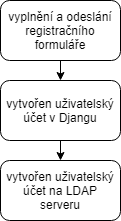
\includegraphics[width=80pt]{./pictures/my_console_current_version_cz.png}
    \caption[Vytváření uživatele - současný stav]{Vytváření uživatele - současný stav (zdroj:
	\href{}{Tereza Kulovaná})}
    \label{fig:admin-current}
\end{figure}
  
V konečné formě by mělo mezi jednotlivými činnostmi probíhat potvrzení přes email. Konkrétně přímo po registraci bude uživateli odeslán email na vyplněnou adresu, který bude nutné před následujícími akcemi potvrdit. Poté bude vytvořen účet v Djangu s neaktivním statusem, který uživateli zabraňuje se do systému přihlásit. Správce obdrží email s žádostí o vytvoření uživatelského účtu, jenž bude přímo obsahovat volby pro potvrzení a zamítnutí. Pokud bude požadavek zamítnut, administrátor vyplní zdůvodnění tohoto rozhodnutí, účet bude z Djanga smazán a uživatel obdrží vysvětlující zprávu. V případě vyhovění žádosti se účet stane aktivním a vytvoří se jeho ekvivalent v \zk{LDAP}. Uživatel bude o kladném rozhodnutí spraven emailem.
  
\begin{figure}[H] \centering
    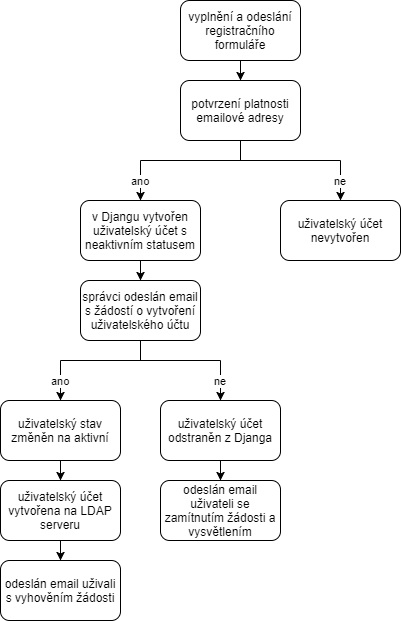
\includegraphics[width=250pt]{./pictures/my_console_final_version_cz.png}
    \caption[Vytváření uživatele - finální stav]{Vytváření uživatele - finální stav (zdroj:
	\href{}{Tereza Kulovaná})}
    \label{fig:admin-final}
\end{figure}

Ověřování platnosti emailové adresy bude doplněno i do části uživatelské konzole, jež umožňuje editaci osobních údajů.

%python knihovna
Vývoj knihovny pro správu uživatelů psané v jazyce Python má počátek v roce 2015. Její vznik byl iniciován především proto, aby nahradila stávající shellové skripty, protože vývojářům GIS.labu je bližší Python a následné úpravy pro ně budou tímto způsobem snadnější. Neméně důležitá je i možnost propojení s webovým rozhraním, a tak byly práce na této knihovně nedávno po delší odmlce obnoveny. 

Aktuálně jsou zpracovány skripty pro tvorbu, úpravu a mazání uživatelských účtů a správu známých zařízení v síti.  Před propojením s webovou konzolí je bude potřeba ještě dokončit a vytvořit nové pro správu skupin (rolí). 
  
% loggování a zprávy
Přes opakované pokusy se nepodařilo zprovoznit vypisování informačních zpráv (tzv. logů) pro úroveň DEBUG, které by usnadnily vývoj. Aktuálně jsou dostupné pouze hlášky pro úroveň INFO a vyšší. Před dalším postupem bude třeba tuto problematiku hlouběji prozkoumat a vyřešit. 

V rámci vlastních funkcí jsou vypisovány informační logy v podobě prostého textu. Ty dostanou vhodnější formátování a budou doplněny o datum a čas, kdy daná činnost proběhla. Pro lepší informovanost o dění budou přidány chybové hlášky. Veškeré informace, které se aktuálně ukazují v konzoli, budou ukládány do souborů.

Administrátorská konzole, která vychází z konzole Djanga, obsahuje informační zprávy, jež se správci zobrazují ve webovém prohlížeči. Tato funkcionalita bude doplněna i pro uživatelskou konzoli. 

% ldap_auth.py
Synchronizace skupin do Djanga je realizována funkcí \textsf{custom\_sync\_user\_relations()}. V rámci úprav kódu se stane členskou metodou nové třídy.

% žádost o role
O role, které budou uživatele opravňovat k využití jednotlivých balíčků GIS.labu, si bude moci uživatel zažádat sám. Nyní se v uživatelské konzoli klient pouze dozví, které role jsou pro něj aktivní. Ve finální verzi si bude moci uživatel vybrat zvolené role během registrace či si o jejich změnu zažádat přes uživatelskou konzoli. Vyhovění či zamítnutí požadavku provede administrátor a uživatel bude informován emailem. Podobně bude implementována i žádost o navýšení kapacity databáze a další služby popsané v kapitole GIS.lab (\ref{vision}). 

%docker
Docker ještě doplním.